\documentclass[../main.tex]{subfiles}
\begin{document}
\section{Anillos y módulos noetherianos}
\begin{proposition}
Sea $A$ un anillo y $M$ un $A$-módulo. Las siguientes afirmaciones son equivalentes.\begin{enumerate}
    \item Todo conjunto no vacío de submódulos de $M$ tiene un elemento maximal respecto del contenido.
    \item Toda sucesión ascendente de submódulos de $M$ $M_1\subset M_2\subset\dots\subset M_n\subset\dots$ es estacionaria, es decir, existe un $k\in\N$ tal que $M_k=M_{k+l}$ para todo $l\in\N$.
    \item Todo submódulo de $M$ es finitamente generado
\end{enumerate}
Si $M$ verifica cualquiera de estas condiciones equivalentes se dice que es un $A$-módulo \textit{noetheriano}. Un anillo $A$ se dice que es un \textit{anillo noetheriano} si, visto como un $A$-módulo, es noetheriano.
\end{proposition}
\begin{proof} Vamos probando cada una de las implicaciones.

($1\Rightarrow 2$) Sea $M_k$ el elemento maximal del conjunto $\{M_n:n\in\N\}$ formado por cada uno de los submódulos de la cadena. Necesariamente, para cada $l\in\N$, $M_k=M_{k+l}$, por ser la cadena ascendente y para no contradecir la maximalidad de $M_k$.

($2\Rightarrow 3$) Sea $N\subset M$ un submódulo arbitrario. Supongamos que $N$ no es finitamente generado. Entonces, $N\neq\{0\}$. Sea $f_1\in N\setminus\{0\}$. Como $N$ no es finitamente generado, $\langle f_1\rangle\varsubsetneq N$. Sea $f_2\in N\setminus\langle f_1\rangle$. Como $N$ no es finitamente generado, $\langle f_1,f_2\rangle\varsubsetneq M$. Inductivamente, generamos una sucesión $\langle f_1\rangle\varsubsetneq\langle f_1,f_2\rangle\varsubsetneq\dots\varsubsetneq\langle f_1,\dots,f_n\rangle\varsubsetneq\dots$ de $A$-módulos no estacionaria, contradiciendo la hipótesis.

($3\Rightarrow 1$) Sea $\Sigma$ un conjunto no vacío de submódulos de $M$, ordenados por la inclusión. Tomemos $\{N_i:i\in I\}$ una cadena de $\Sigma$. Definiendo $N^{\ast}=\bigcup_{i\in I}N_i\subset M$. Por hipótesis, $N^{\ast}$ es finitamente generado. Sean $y_1,\dots,y_l$ sus generadores. Supongamos que cada $y_j\in N_{i_j}$. Sea $N_k=\operatorname{max}\{N_{i_1},\dots,N_{i_l}\}$. Como $\{N_i\}$ es una cadena, necesariamente se tiene $N^{\ast}=N_k$.

Hemos visto que toda cadena de $\Sigma$ tiene máximo. Por el Lema de Zorn, $\Sigma$ tiene elemento maximal.
\end{proof}
\begin{proposition}
Dada una sucesión corta y exacta de homomorfismos de $A$-módulos $$0\longrightarrow M'\overset{f}{\longrightarrow}M\overset{g}{\longrightarrow}M''\longrightarrow 0$$ $M$ es noetheriano si y solo si $M'$ y $M''$ son noetherianos.
\end{proposition}
\begin{proof} Utilizamos las diferentes caracterizaciones de los $A$-módulos noetherianos descritas en la proposición anterior.

($\Longrightarrow$) Una cadena ascendente de submódulos de $M'$ lo es también de $M$ por ser $f$ inyectiva. Usando $(2)$, dicha cadena es estacionaria y por tanto $M'$ es noetheriano.

Como $g$ es sobreyectiva, $M''\cong\faktor{M}{\operatorname{ker} g}$. Por el Teorema de la correspondencia, los submódulos de $\faktor{M}{\operatorname{ker} g}$ son de la forma $\faktor{T}{\operatorname{ker} g}$ con $T\supset \operatorname{ker} g$ un submódulo de M. Como M es noetheriano, por $3$, $T$ es finitamente generado y por tanto, $\faktor{T}{\operatorname{ker} g}$ también y $M''$ es noetheriano.

($\Longleftarrow$) Sea $N\subset M$ un submódulo. $f^{-1}(N)$ es un submódulo de $M'$, luego es finitamente generado. Sean $x_1,\dots,x_r$ sus generadores. Usando que $M''\cong\faktor{M}{\operatorname{ker} g}$, $\faktor{(N+\operatorname{ker} g)}{\operatorname{ker} g}$ es un submódulo de $M''$ y entonces es finitamente generado. Sean $\overline{y_1},\dots,\overline{y_k}$ sus generadores. Veamos que $\langle f(x_1),\dots,f(x_r),y_1,\dots,y_k\rangle$ generan $N$.

Dado $z\in N$, existen $\lambda_i\in A$, $i=1,\dots,k$ tal que $$\overline{z}=\sum_{i=1}^k\lambda_i\overline{y_i}$$ Se tiene que $w=z-\sum_{i=1}^k\lambda_iy_i\in\operatorname{ker} g=\operatorname{Im} f$, luego existe $u\in M'$ tal que $f(u)=w$. Existen $\mu_j\in A$, $j=1,\dots,r$ tal que $u=\sum_{j=1}^r\mu_jx_j$. Aplicando $f$, se cumple $$w=\sum_{j=1}^r\mu_jf(x_j)$$ Con todo se tiene que $$z=\sum_{j=1}^r\mu_jf(x_j)+\sum_{i=1}^k\lambda_iy_i$$
\end{proof}
\begin{remark}
De este resultado se siguen las siguientes consecuencias.\begin{enumerate}
    \item Los cocientes y submodulos de los $A$-módulos noetherianos son noetherianos.
    \item Si $M_1,\dots,M_r$ son $A$-módulos noetherianos, $\bigoplus_{i=1}^rM_i$ es noetheriano.
    \item Sea $M$ un $A$-módulo finitamente generado, donde $A$ es un anillo noetheriano. Entonces $M$ es un $A$-módulo noetheriano. En efecto, si $r$ es un número de generadores de $M$, por ser $A$ noetheriano, $A^{(r)}$ es noetheriano también y se genera la sucesión exacta $A^{(r)}\rightarrow M\rightarrow 0$.
    \item Si $A$ es un anillo noetheriano, entonces cualquier localización suya lo es. Para ver esto, sea $\af'\in\S^{-1}A$ un ideal. Sabemos que existe $\af\subset A$ tal que $\af^e=\af'.$ Como $\af$ es finitamente generado, digamos por $\{x_1,\dots,x_s\}$, entonces $\{\frac{x_1}{1_A},\dots,\frac{x_s}{1_A}\}$ será un sistema de generadores finito de $\af'.$
\end{enumerate}
\end{remark}
El Teorema de la base de Hilbert del primer capítulo nos garantiza que si $A$ es un anillo noetheriano, $A[X]$ es también noetheriano. Inductiavente se ve que $A[X_1,\dots,X_n]$ es también noetheriano.

A su vez, si recordamos la definición de $A$-álgebra finitamente generada del primer capítulo, se tiene que existe un homomorfismo suprayectivo de $A[X_1,\dots,X_n]$ en $B$, donde $B$ es la $A$-álgebra y $n$ es el número de generadores de $B$ como $A$-álgebra. Entonces, si $A$ es un anillo noetheriano, cualquier $A$-álgebra finitamente generada es un anillo noetheriano.

\section{Asociados primos y descomposición primaria}
Sea $A$ un anillo noetheriano y $\af$ un ideal. El objetivo de esta sección es descomponer $\af$ como intersección finita $\af=\bigcap \q_i$, con cada $\q_i$ primario asociado a un ideal primo $\p_i$.

Buscamos que tal descomposición sea \textit{irredundante}. Esto es que para cada $i$ se verifique $\q_i\nsupseteq \bigcap_{j\neq i}\q_j$.

En $\faktor{A}{\af}$, esto es equivalente a hacer la descomposición sobre el $0$ de $\faktor{A}{\af}$.

\begin{remark}
\begin{enumerate}
    \item Tal descomposición no tiene por qué ser única. Si tomamos por ejemplo en el anillo $A=K[X,Y]$ el ideal $\af=\langle x^2,xy\rangle$, se cumple $\af=\langle x\rangle\cap\langle x^2,y=\langle x\rangle\cap\langle x^2,xy,y^2\rangle$.
    \item  Veremos más adelante que los asociados primos sí son únicos. En el caso anterior serían $\langle x\rangle, \langle x,y\rangle$.
\end{enumerate}
\end{remark}
Siguiendo con lo anterior, supongamos que tenemos una descomposición irredundante del ideal $0$ en ideales primarios. Esto es, $\langle 0\rangle=\bigcap_{i=1}^r\q_i$, donde $\q_i$ es un ideal que verifica que $\sqrt{\q_i}=\p_i$, siendo $\p_i$ un ideal primo para cada $i=1,\dots,r$. Dado $x_i\in\cap_{j\neq i}\q_j\setminus\q_i$, que existe por ser la descomposición irredundante, supongamos que existe $\lambda\in A$ tal que $\lambda x_i=0$. Entonces, como $x_i\notin\q_i$, que es primario, necesariamente $\lambda\in\sqrt{\q_i}=\p_i$. Es decir, $\operatorname{anul}_A(x_i)\subset\p_i$. Además, para cada $\mu\in A$, $\operatorname{anul}_A(x_i)\subset\operatorname{anul}_A(\mu x_i)\subset\p_i$.

Tomando $\Sigma=\{\operatorname{anul}_A(x):x\in A\setminus\{0\}\}$, este conjunto tiene elementos maximales. Sea $\operatorname{anul}_A(z)$ uno de ellos. Si suponemos que existen $\lambda,\mu\in A$ tales que $\lambda\mu\in\operatorname{anul}_A(z)$, es decir, $\lambda\mu z=0$ y además $\mu\notin\operatorname{anul}_A(z)$, entonces $\mu z\neq0$. Esto significa que $\operatorname{anul}_A(z)\subset\operatorname{anul}_A(\mu z)\in\Sigma$. Por maximalidad, como $\lambda\in\operatorname{anul}_A(\mu z)$, se tiene que cumplir que $\lambda\in\operatorname{anul}_A(z)$. Acabamos de ver que $\operatorname{anul}_A(z)$ es primo. Esto motiva la siguiente definición.
\begin{definition}
Sea $M$ un $A$-módulo. Se denominan \textit{primos asociados} de $M$ a los ideales primos de la forma $\operatorname{anul}_A(x)$ para algún $x\in M$. El conjunto de estos se denota $Ass_AM$.
\end{definition}
\begin{definition}
Sea $M$ un $A$-módulo. Llamamos \textit{soporte} de $M$ y lo denotamos por $\operatorname{supp} M$ al conjunto de los ideales primos $\p$ de $A$ tales que $M_{\p}\neq 0$.
\end{definition}
\begin{lemma}
\begin{enumerate}
    \item Si $M\neq\{0\}$, entonces $\Ass_AM\neq\varnothing$.
    \item Si $M\cong M'$, entonces $\Ass_AM=\Ass_AM'$.
    \item $\Ass_AM\subset\operatorname{supp}M$.
\end{enumerate}
\end{lemma}
\begin{proof}
  3. Sea $\mathfrak{p}\in \Ass_A M$, entonces existe un $x\in M$ tal que $\mathfrak{p} = \anul_A(x)$. Si en la localización $M_\mathfrak{p}$ se tuviese $\frac{x}{1} = 0$, entonces existiría $s\in A\setminus \mathfrak{p}$ tal que $sx = 0_M$, es decir, $s\in \anul_A(x)$ pero $ \anul_A(x) \setminus \mathfrak{p} = \varnothing$.
\end{proof}

\begin{proposition}
Sea $A$ un anillo noetheriano. Entonces,\begin{enumerate}
    \item $\bigcup_{\p\in\Ass_AM}\p=\operatorname{Div}_0M$.
    \item Si $S\subset A$ es un conjunto multiplicativamente cerrado, entonces $\Ass_{S^{-1}A}(S^{-1}M)=\Ass_A(M)\cap\{\p\in\operatorname{Spec(A):\p\cap S=\varnothing}\}$.
\end{enumerate}
\end{proposition}

\begin{proof}
Comencemos con $i)$. El contenido $\subset$ se tiene por la propia definición de $\operatorname{Ass}_A(M)$. Para $\supset$, sea $\lambda\in A$ ral que $\lambda x=0$ para $x\in M\setminus\{0_M\}.$ Sea
$$\Sigma:=\{\operatorname{anul}_A(\mu x)\ :\ \mu\in A,\ \mu x\neq 0_M\},$$
que es un conjunto no vacío de ideales de $A$ y todos ellos contienen a $\operatorname{anul}_A(x).$

Como $A$ es noetheriano, $\Sigma$ contiene ideales maximales: consideremos uno de ellos, $\af:=\operatorname{anul}_A(\alpha x).$ Si $\beta\gamma\in\af$ y $\beta\notin\af$, entonces $\beta\alpha x\neq 0_M$ y $\gamma\in\operatorname{anul}_A(\beta\alpha x)\supset\operatorname{anul}_A(\alpha x)=\af.$ Por la maximalidad de $\af$, ambos son iguales y $\gamma\in\af.$ Así, $\af\in\Ass_A(M)$ y $\anul_A(x)\subset\af.$

Probemos ahora $ii).$ Sabemos que existe una biyección
$$\{\p\in\Spec A\ :\ \p\cap S=\varnothing\}\leftrightarrow\Spec{S^{-1}A}.$$
Como los elementos $s\in S$ son unidades en $S^{-1}A$ vistos como $\frac{s}{1}$, es suficiente probar que para todo $\p\in\Spec A$ tal que $\p\cap S=\varnothing$ y para toda $x\in M\setminus\{0_M\}$ se tiene
$$\p=\anul_A(x)\Leftrightarrow \p^e=\anul_{S^{-1}A}\left(\frac{x}{1}\right).$$ Esto es así porque, dado un elemento $\frac{x}{s}\in S^{-1}M$, $\anul_{S^{-1}A}(\frac{x}{s})=\anul_{S^{-1}A}(\frac{x}{1})$ por ser $\frac{1}{s}$ unidad en $S^{-1}A.$

$(\Rightarrow)$ Veamos el contenido $\supset$. Si $\frac{\gamma x}{s 1}=0_{S^{-1}M}$, existe $s'\in S$ tal que $s'\gamma x=0_M$. De esta forma, $\lambda:=s'\gamma\in\p$ y $\frac{\gamma}{s}=\frac{\lambda}{ss'}\in\p^e.$ Para $\subset$, un elemento de $\p^e$ es de la forma $\frac{\alpha}{t}$, donde $\alpha\in\p$ y $t\in A\setminus S.$ Como $\alpha x=0_M$, $\frac{\alpha}{t}\frac{x}{1}=0_{S^{-1}M}.$

$(\Leftarrow)$ Si $\lambda\in A$ verifica $\lambda x=0_M$, $\frac{\lambda}{1}\in\anul_{S^{-1}A}(\frac{x}{1})$ y $\lambda\in\p^{ec}=\p;$ es decir, $\anul_A(x)\subset\p.$ Por otro lado, si $\lambda\in\p$, $\frac{\lambda}{1}\in\p^e,$ por tanto $\frac{\lambda x}{1}=0_{S^{-1}M}$ y existe $s'\in S$ tal que $s'\lambda x=0_M.$ Así, $s'\lambda\in\anul_A(x)\subset\p$ y como $s'\notin\p$, $\lambda\in\p.$

\end{proof}

\begin{lemma}\label{contenidos_assa}
Sea $A$ un anillo noetheriano, si la sucesión $$0\overset{f}{\longrightarrow} M'\longrightarrow M\overset{g}{\longrightarrow} M''\longrightarrow 0$$ es exacta, entonces se cumple $$\Ass_A(M')\subset\Ass_A(M)\subset\left (\Ass_A(M'')\cup\Ass_A(M')\right )$$ y se tiene la igualdad si la sucesión es escindida.
\end{lemma}\label{contenidos_assa}
\begin{proof}
El primer contenido se tiene porque si $\mathfrak{p}$ es anulador de $x \in M'$, entonces para todo $a \in \mathfrak{p}$ tenemos que $af(x)  f(ax) = f(0_{M'}) = 0_M$, luego $\mathfrak{p}$ es anulador de $f(x)$.

Para el segundo, distinguimos entre los elementos que pertenecen a $\ker g$ y los que no. Si $z\in\ker(g)= \im(f)$, entonces existe $z'\in M'$ con $z=f(z')$ y por la inyectividad de $f$ se tiene $0 = af(z') = f(az')$ si y solo si $az' = 0 $, luego $\anul_A(z)=\anul_A(z')$ y así si $\mathfrak{p}\in \Ass_A(M)$ es el anulador de un elemento de $\ker g$, pertenece a $\Ass_A(M')$. Tomemos ahora $\mathfrak{p}\in \Ass_A(M) \setminus \Ass_A(M') $ y sea $x\in M\setminus \ker g$ tal que $\mathfrak{p} = \anul_A(x)$.

Llamamos $x'':=g(x)\neq 0_{M''}$ y vamos a ver que $\anul_A(x)=\anul_A(x'')$. Por la linealidad, $\anul_A(x) \subset \anul_A(x'')$. Supongamos, por reducción al absurdo, que el contenido es estricto y sea $b \in\anul_A(x'')\setminus\anul_A(x)$. Tenemos que $0_{M''} = b x''=g(b x)$ luego $bx \in \ker g = \im f$ y asi existe $x'\in M'\setminus\{0_{M'}\}$ tal que $f(x')=b x$.
Como hemos visto antes $\anul_A(x')=\anul_A(b x)\supset\anul_A(x)=\p$ y como $\p\notin\Ass_A(M')$ el contenido es estricto. Por lo tanto, existe $\alpha \in \anul_A(b x) \setminus\anul_A(x) $, es decir, tal que $\alpha x\neq 0_M$ y $\alpha b x=0_M$, de donde $\alpha b\in \anul_A(x) = \p$, pero $\alpha,\mu\notin\p$, lo que contradice la primalidad de $\mathfrak{p}$.
\end{proof}

\begin{proposition}\label{cadena_assa}
Sea $A$ un anillo noetheriano y $M$ un $A$-módulo no vacío finitamente generado. Entonces, existe una sucesión ascendente de submódulos $$\{0_M\}=:M_0\subset M_1\subset\dots\subset M_{n-1}\subset M_n:=M$$ con $\Ass_A(M_i/M_{i-1})=\p_i$ para cada $i=1,\dots,n$.

En particular, $\Ass_AM\subset\{\p_1,\dots,\p_n\}$ es finito.
\end{proposition}

\begin{proof}
Como $M\neq\{0\}$, existe $\p_1\in\Ass_A(M)\neq\varnothing$ y $\p_1=\anul_A(x_1)$ para cierto $x_1\in M.$ Sea el submódulo que genera\footnote{Al igual que en espacios vectoriales, se trata de todos los múltiplos $\lambda x_1$ con $\lambda\in A$.}
$M_1:=\langle x_1\rangle\subset M$. Podemos definir un homomorfismo de $A$-módulos $A\to M_1$ dado por $1_A\mapsto x_1$, y el núcleo es $\mathfrak{p}_1$ por lo que tenemos el isomorfismo $M_1\cong A/{\p_1}$. En $A/{\p_1}$ está claro que los únicos anuladores son los elementos de $\mathfrak{p_1}$ y así $\Ass_A(M_1)=\Ass_A(A/\mathfrak{p}_1) = \{\p_1\}$.
Por el lema anterior $\Ass_A(M)\subset \left ( \Ass_A(M_1)\cup\Ass_A{(M/M_1) } \right).$

Si $M/M_1\neq 0$, existe $\p_2\in\Ass_A(M/M_1)$ de la forma $\p_2=\anul_A(x_2+ M_1)$ para cierto $x_2+ M_1\in M/M_1$ no nulo. De nuevo, consideramos el submódulo generado, que por el teorema de la correspondencia es de la forma $\langle x_2 + M_2 \rangle =: M_2/M_1$ para algún submódulo $M_2\subset M$ con $M_1\subset M_2$. Procediendo como antes, $A/{\p_2}\cong M_2/M_1$ y llegamos a que $\Ass_A(M_2/M_1)=\{\p_2\}$.
Tenemos la sucesión exacta
\begin{equation}
  0 \to \faktor{M_2}{M_1} \to \faktor{M}{M_1} \to \faktor{M/M_1}{M_2/M_1} = \faktor{M}{M_2}  \to 0
\end{equation}

de manera que $\Ass_A(M/M_1) \subset \left (\Ass_A (M_2/M_1) \cup \Ass_A(M/M_2) \right )$, y sustituyendo en lo de antes sacamos que $\Ass_A(M)\subset \{\p_1\}\cup\{\p_2\}\cup\Ass_A(M/M_2)$. Reiterando el proceso obtenemos una sucesión, $\{0\}\subset M_1\subset M_2\cdots$, que se estabiliza por ser $M$ noetheriano, es decir, existe $n\in\N$ tal que $M_n=M.$
\end{proof}

\begin{definition} Sea $M$ un $A$-módulo. \begin{enumerate}
    \item Un submódulo $N\varsubsetneq M$ se dice \textit{submódulo primario asociado} al ideal primo $\p$ si $\Ass_A(M/N)=\{\p\}$.
    \item Un submódulo $N\subset M$ distinto del $0$ se dice \textit{irreducible} si $N=N_1\cap N_2$ implica que $N=N_1$ ó $N=N_2$.
\end{enumerate}
\end{definition}

\begin{lemma}
Sea $A$ un anillo noetheriano y $M$ un $A$-módulo. Entonces,\begin{enumerate}
    \item Si $N_1$ y $N_2$ son dos submódulos primarios asociados a un mismo ideal primo, entonces $N_1\cap N_2$ cumple esta propiedad también.
    \item Todo submódulo irreducible es primario.
\end{enumerate}
\end{lemma}

\begin{proof}
$(i)$ Tenemos por hipótesis $\Ass_A(M/N_i)=\{\p\}$ para $i\in\set{1,2}$ y
$$\begin{array}{rcl}
    M&\longrightarrow& M/N_1\oplus M/N_2\\
    x&\longmapsto&(x\operatorname{mod}  N_1,x\operatorname{mod} N_2)
\end{array}$$
induce una sucesión
$$0\longrightarrow M/(N_1\cap N_2)\longrightarrow M/N_1\oplus M/N_2$$
exacta. Así, $\varnothing\neq \Ass_A(M/(N_1\cap N_2))\subset \{p\}$ y $N_1\cap N_2$ es $\p$-primario.

$(ii)$ Sea $\{0\}\neq N\subsetneq M$ un submódulo y supongamos que $N$ no es primario para comprobar que tampoco es irreducible. Como no es el 0 existe algún $\p_1\in\Ass_A(M/N)$ y por la proposición \ref{cadena_assa} existe un submódulo de $N_1 / N \subset M/N$ tal que $\Ass_A(N_1/N)=\{\p_1\}$.
Ahora, como $N$ no es primario, existe $\p_2\in\Ass_A(M/N)$ distinto de $\p_1$ y como antes existe $N_2 / N \subset N_1/N$  con $\Ass_A(N_2/N)=\{\p_2\}.$
Entonces, utilizando el lema \ref{contenidos_assa} podemos ver que
$$\Ass_A((N_1\cap N_2)/N)\subset\Ass_A(N_1/N)=\{\p_1\}$$
y
$$\Ass_A((N_1\cap N_2)/N)\subset\Ass_A(N_2/N)=\{\p_2\}.$$
pero esto implica $\Ass_A((N_1\cap N_2)/N)=\varnothing$ y por lo tanto $(N_1\cap N_2)/N = 0$, es decir, $N_1\cap N_2=N$ y como $N_i\supsetneq N$ llegamos a que $N$ es reducible.
\end{proof}

\begin{lemma}
Sea $A$ un anillo noetheriano, $M$ un $A$-módulo finitamente generado. Entonces todo submódulo de $M$ es una intersección de submódulos irreducibles
\end{lemma}
\begin{proof}
Sea $\Sigma$ el conjunto formado por submódulos propios $Q\subset M$ que no son intersección de submódulos irreducibles. Si $\Sigma=\varnothing$, todos los irreducibles son primarios. Supongamos entonces que $\Sigma\neq\varnothing.$

Como $M$ es noetheriano, $\Sigma$ contiene submódulos maximales. Sea $Q_0\in\Sigma$ uno de ellos. Por definición de $\Sigma$, existen $N_1$ y $N_2$ submódulos de $M$ tales que $Q_0\subsetneq N_i$ y $N_1\cap N_2=Q_0.$ Si suponemos $N_1=M$, entonces $N_2=N_1\cap N_2=Q_0$, que es absurdo. Así, $N_1$ y $N_2$ son submódulos propios y, por la maximalidad de $Q_0$, ambos son intersección finita de submódulos irreducibles; sin embargo, esto es absurdo puesto que en tal caso $Q_0$ también lo sería.
\end{proof}

El lema nos dice que, en particular, todo submódulo $N \subset M$ se escribe como intersección de submódulos primarios. Así ya tenemos probada la existencia de una descomposición primaria que podemos refinar hasta obtener una irredundante.

\begin{theorem} (\textbf{de Lasker-Noether}).
Sean $A$ un anillo noetheriano y $M$ un $A$-módulo finitamente generado. Sea $N\varsubsetneq M$ un submódulo de $M$. Entonces, existen $N_1,\dots,N_r$ submódulos primarios de $M$ asociados a ideales primos $\p_1,\dots,\p_r$, respectivamente, tales que $N=\cap_{j=1}^rN_j$, cada $N_i\varsupsetneq\cap_{j\neq i}N_j$ y $\Ass_A(M/N)=\{\p_1,\dots,\p_r\}$.
\end{theorem}

\begin{proof}
Solo tenemos que desmotrar que, si $N=\bigcap_{i=1}^rN_i$ es una descomposición primaria irredundante, donde cada $N_i$ es $\p_i$-primario, entonces $\Ass_A(M/N)=\set{\p_1,\cdots,\p_r}.$

Para ver el contenido $\subset$ nos valemos del lema \ref{contenidos_assa}. Primero vemos que tenemos el siguiente homomorfismo inyectivo
$$\faktor{M}{N}\hookrightarrow\oplus_{i=1}^r\faktor{M}{N_i}$$
Esá bien definido y es inyectivo porque
\begin{align}
  x + N = y+N & \Rightarrow & x-y \in N = \bigcap N_i & \Rightarrow & x-y \in N-i & \Rightarrow & x+N_i = y+N_i
\end{align}
esto nos dice que $ \Ass_A (M/N) \subset \Ass_A(\oplus_{i=1}^rM/{N_i})$. Queremos ver ahora que este último coincide con $\bigcup_{i=1}^r\Ass_A(M/{N_i})$. De nuevo, usando el lema \ref{contenidos_assa} vemos rápido que como $M/N_i \hookrightarrow \bigoplus M/N_i$ entonces $\Ass_A (M/N_j) \subset \Ass_A (\bigoplus_i M/N_i)$ para todo $j$ y por tanto la unión también está contenida.
Por otra parte, si $\mathfrak{p}\in  \Ass_A (\bigoplus_i M/N_i)$, existen $x_i \in M$ para todo $i$ tales que $\mathfrak{p} = \anul_A(x_1+N_1, \dots, x_n+N_n)$, es decir, que es anulador de cada $x_i+N_i$, luego $\mathfrak{p} \in  \Ass_A (M/N_i)$ para todo $i$, lo que nos da el otro contenido.

Para ver el contenido $\supset$ vamos a demostrar que, uno por uno, cada $\mathfrak{p_i}$ pertenece a $\Ass_A(M/N)$. Consideramos el homomorfismo
$$\begin{array}{rcl}
    N_2\cap\cdots\cap N_r&\overset{f}{\longrightarrow}&M/N_1\\
    x&\longmapsto&x+N_1
\end{array}$$

que tiene por núcldeo a $\bigcap_{i=1}^r N_i = N$. Entonces, nuevamente por el lema \ref{contenidos_assa}, como $(N_2\cap\cdots\cap N_r)/N\hookrightarrow M/{N_1}$ es inyectiva obtenemos $\Ass_A((N_2\cap\cdots\cap N_r)/N) \subset \Ass_A(M/N_1) = \set{\p_1}$, y tenemos la igualdad porque $N_2\cap\cdots\cap N_r)/N \neq 0$ luego $\Ass(N_2\cap\cdots\cap N_r)/N) \neq \varnothing$.
Finalmente, como $(N_2\cap\cdots\cap N_r)/N \subset M/N$, una vez más por el lema \ref{contenidos_assa} tenemos el contenido  $\set{\p_1}= \Ass(N_2\cap\cdots\cap N_r)/N) \subset\Ass_A(M/N)$.

Podemos repetir este argumento para cada $i\in\set{1,\dots,r}$ y así se concluye que $\set{\p_1,\dots,\p_r}\subset\Ass_A(M/N)$.
\end{proof}

\begin{definition}
    Sea $A$ un anillo y $M$ un $A$-módulo, se define $\operatorname{anul}_A(M)$ como el ideal de los $\lambda\in A$ tales que $\lambda x=0_M$ para todo $x\in M$.
\end{definition}

\begin{remark}\textbf{{Relación entre $\supp M, V(\anul_A M)$ y $\Ass_A M$}}

Sea $\p\subset A$ un ideal primo y supongamos que existe $\lambda\in(\anul_A M)\setminus\p$; por ser así, para todo $x\in M$ se tendría $\lambda x=0_M$, es decir, $\frac{x}{1}=0_{M_\p}$ y $\p\notin\supp M.$ Tras esto tenemos que
$$\supp M\subset V(\anul_A M)=\{\p\subset A\ :\ \p\supset\anul_A M\}.$$

Más aún, si $M$ es finitamente generado, se tiene la igualdad. Para ver esto, tomemos $\p\notin\supp M$, es decir, $M_\p=\{0\}.$ Sean $x_1,\dots,x_s$ los generadores de $M$, por la igualdad $M_\p=\{0\}$ tenemos que existe $\lambda_i\notin\p$ para cada $i\in\{1,\dots,s\}$ de forma que $\lambda_i x_i=0_M.$ Definiendo $\lambda:=\prod_{i=1}^s\lambda_i,$ $\lambda\in\anul_A M$ pero $\lambda\notin\p$; es decir, $\anul_A M\not\subset\p$ y $\supp M\supset V(\anul_A M)=\{\p\subset A\ :\ \p\supset\anul_A M\}.$

% \begin{remark}
% Por definición del anulador tenemos que
% $$
% \anul_A M = \bigcap_{x\in M} \anul_A(x) = \bigcap_{\mathfrak{p} \in }
% $$
%
% \end{remark}

\begin{lemma}\label{min_supp}
Sea $A$ un anillo noetheriano y $\p\in\supp M$ minimal en $\supp M$. Bajo estas hipótesis, $\p\in\Ass_A M.$
\end{lemma}
\begin{proof}
Tomemos $\p\in\supp M.$ Ya sabemos $A_\p$ es noetheriano por serlo $A.$ En este caso, nuestro conjunto multiplicativamente cerrado es $A\setminus\p$ y por esto, para cada $\p'\in\Spec A$, se tiene
$$\p'\cap S=\varnothing\Leftrightarrow \p'\subset\p.$$
Así, resulta la biyección
$$\Ass_{A_\p}(M_\p)\leftrightarrow\Ass_A(M)\cap\{\p'\in\operatorname{Spec(A):\p'\subset\p}\}.$$
Sea ahora $\p$ verificando las hipótesis del lema.  Como $M_\p\neq\{0\}$, $\Ass_{A_\p} M_\p\neq\varnothing$ y existe $\p'\in \Ass_A(M)\cap\{\p'\in\operatorname{Spec(A):\p'\subset\p}\}$ por lo que acabamos de ver. De esta forma, la minimalidad de $\p$ en $\supp M$ nos permite concluir que $\p\subset\p'$ y $\p\in \Ass_A M.$
\end{proof}

Por el lema tenemos que todos los primos minimales de $\supp M$ son elementos de $\Ass_A M$, y como sabemos que $\Ass_A M \subset \supp M$, en particular son minimales entre los elementos $\Ass_A M$, así que si tomamos un minimal en $\Ass_A M$ tiene que ser minimal de $\supp M$. Esto completa la prueba de que $\operatorname{min}(\Ass_A M) = \operatorname{min}(\supp M)$.

Más aún, en el caso de un módulo finitamente generado, como puede ser un anillo de polinomios y sus cocientes por ideales, tenemos por el desarrollo anterior que también ha de coincidir con $\operatorname{min}(V(\anul_A(M)))$.

\end{remark}

\begin{figure}


\tikzset{every picture/.style={line width=0.75pt}} %set default line width to 0.75pt

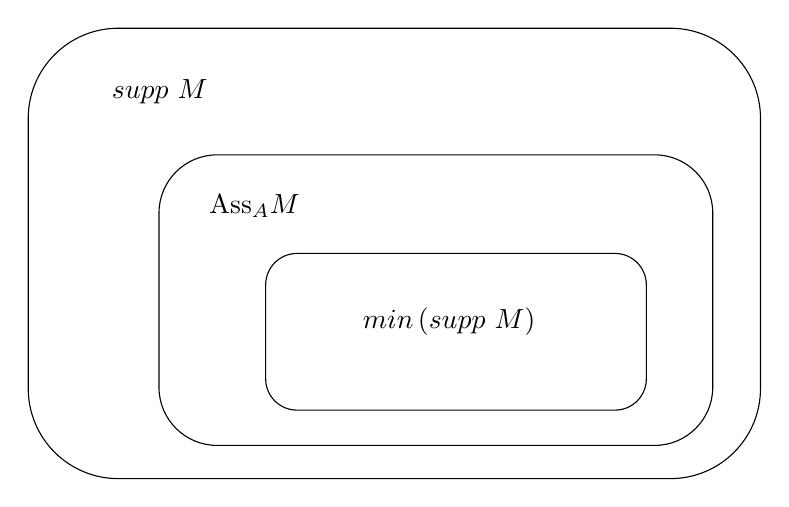
\begin{tikzpicture}[x=0.75pt,y=0.75pt,yscale=-1,xscale=1]
%uncomment if require: \path (0,300); %set diagram left start at 0, and has height of 300

%Rounded Rect [id:dp7938091256043489]
\draw   (154,83.4) .. controls (154,59.43) and (173.43,40) .. (197.4,40) -- (463.4,40) .. controls (487.37,40) and (506.8,59.43) .. (506.8,83.4) -- (506.8,213.6) .. controls (506.8,237.57) and (487.37,257) .. (463.4,257) -- (197.4,257) .. controls (173.43,257) and (154,237.57) .. (154,213.6) -- cycle ;
%Rounded Rect [id:dp6376671037251953]
\draw   (217,129) .. controls (217,113.54) and (229.54,101) .. (245,101) -- (455.8,101) .. controls (471.26,101) and (483.8,113.54) .. (483.8,129) -- (483.8,213) .. controls (483.8,228.46) and (471.26,241) .. (455.8,241) -- (245,241) .. controls (229.54,241) and (217,228.46) .. (217,213) -- cycle ;
%Rounded Rect [id:dp8227299140826816]
\draw   (268.4,163.6) .. controls (268.4,155.26) and (275.16,148.5) .. (283.5,148.5) -- (436.7,148.5) .. controls (445.04,148.5) and (451.8,155.26) .. (451.8,163.6) -- (451.8,208.9) .. controls (451.8,217.24) and (445.04,224) .. (436.7,224) -- (283.5,224) .. controls (275.16,224) and (268.4,217.24) .. (268.4,208.9) -- cycle ;

% Text Node
\draw (193,63.4) node [anchor=north west][inner sep=0.75pt]    {$\text{supp} \ M$};
% Text Node
\draw (240,119) node [anchor=north west][inner sep=0.75pt]   [align=left] {Ass$\displaystyle _{A}$$\displaystyle M$};
% Text Node
\draw (314,173.4) node [anchor=north west][inner sep=0.75pt]    {$\text{min}\left(\text{supp} \ M\right)$};


\end{tikzpicture}
  \caption{}
\end{figure}

\begin{theorem}
Sea $A$ un anillo noetheriano y sea $M$ un $A$-módulo finitamente generado.\begin{enumerate}
    \item Sea $N\subset M$ un submódulo $\p$-primario y sea
    $$\begin{array}{rrcl}
	\nu:&M&\longrightarrow&M_{\p}\\
	&x&\longmapsto&\frac{x}{1}\\ \end{array}$$ Entonces, $\nu^{-1}(N_{\p})=N$.
	\item Sea $N\subset M$ y sea $N=\cap_{i=1}^rQ_i$ una descompsición irredundante en submódulos $\p_i$-primarios para cada $i=1,\dots,r$, cumpliéndose que $\Ass_A(M/N)=\{\p_1,\dots,\p_r\}$. Si $\p_j$ es un ideal minimal en $\Ass_A(M/N)$ y $\nu_j:M\longrightarrow M_{\p_j}$, entonces $Q_1=\nu_j^{-1}(N_{\p_j})$.

	Esto significa que los ideales primarios que aparecen en la descomposición irredundante de un submódulo de $M$ y corresponden a ideales primos asociados minimales están unívocamente determinados.
\end{enumerate}
\end{theorem}
\begin{proof}
\textit{1.} Sabemos que si $N\subset M$ es un submódulo, entonces $N_{\p}\subset M_{\p}$ es submódulo de manera que podemos tomar la preimagen $N':=\nu^{-1}(N_{\p})$ que es un submódulo de $M$ que contiene a $N$ y el enunciado tiene sentido.

Vamos a ver que $N'/N = 0$. Tenemos que $N'/N\subset M/N$ es un submódulo por tanto $\Ass_A(N'/N)\subset\Ass_A(M/N)=\{\p\}$ pues $N$ es $\p$-primario. Además, sabemos que $\Ass_A(N'/N)\subset\supp\{(N'/N)\}$.
Ambas cosas juntas dan que $\Ass_A(N'/N) \subset \left ( \{p\}\cap\supp(N'/N) \right).$ Si probamos que $\p\notin\supp(N'/N)$, ie. $(N'/N)_\p = 0$, tendremos que $\Ass_A(N'/N)=\varnothing$ y así $N'/N=0$ luego $N' = N$.

Como $N \subset N'$, se tiene $N_\p \subset (N')_\p$. Además, $(N')_{\p} \subset N_{\p}$ ya que si $\frac{m}{t}\in (N')_\p$,
entonces $m \in N' = \nu ^{-1} (N_\p)$ y así $\frac{m}{1} \in N_\p$, lo que quiere decir que $m \in N$, y por lo tanto $\frac{m}{t} \in N_\p$. Así hemos probado que $(N')_\p = N_\p$ y por el corolario \ref{cociente_localiza} se tiene $(N'/N)_\p \cong (N')_\p / N_\p = 0$ como queríamos ver.

\textit{2.} Sin pérdida de generalidad trabajamos con $j=1$. En primer lugar, comprobamos que $\nu_1:M\longrightarrow M_{\p_1}$ conserva las intersecciones. Sean $N'$ y $N''$ submódulos de $M$. La inclusión $(N'\cap N'')_{\p_1}\subset {N_{\p_1}}'\cap{N_{\p_1}}''$ es clara. Por otro lado, dado un elemento $\omega\in {N_{\p_1}}'\cap{N_{\p_1}}''$, existen $n'\in N'$, $n''\in N''$ y $t,s\notin\p_1$ tales que $\omega=\frac{n'}{s}=\frac{n''}{t}.$ Por esto, también existe $\lambda\notin\p_1$ tal que $\lambda tn'=\lambda sn''=:\eta$; es decir, $\eta\in N'\cap N''$ y $\omega=\frac{\eta}{\lambda ts}.$ Es por esto que, si $N=\cap_{i=1}^r Q_i$, entonces $N_{\p_1}=\cap_{i=1}^r(Q_i)_{\p_1}.$

Si comprobamos que $(Q_i)_{\p_1}=M_{\p_1}$ para todo $i\neq 1$, habremos terminado porque la intersección se reducirá a $(Q_1)_{\p_1}$ y por el apartado anterior $v_1^{-1}((Q_1)_{\p_1}) = Q_{\p_1}$.
Para cada $i\neq 1$ usamos la biyección del lema \ref{min_supp}:
$$\Ass_{A_{\p_1}}((M/Q_i)_{\p_1})\leftrightarrow\Ass_A(M/Q_i)\cap\{\p'\in\operatorname{Spec(A):\p'\subset\p}\}.$$

Por hipótesis $\Ass_A(M/Q_i)=\{\p_i\}$ y también por hipótesis $\p_j\not\subset\p_1$ pues este último es minimal en $\Ass(M\setminus N)$. Entonces, para cada $i\neq 1$ se tiene que  $\Ass_A{A_{\p_1}}((M/Q_i)_{\p_1})=\varnothing$.
\end{proof}


\begin{proposition}
Sea $A$ un anillo noetheriano, $S\subset A$ un conjunto multiplicativamente cerrado, $M$ un $A$-módulo y $N=\cap_{i=1}^rN_i \subset M$  un submódulo descompuesto en submódulos $\p_i$-primarios. Entonces, $S^{-1}N_i$ es un $S^{-1}$-submódulo primario de $S^{-1}M$ si y solo si $S\cap\p_i=\varnothing$.

En el caso contrario, $S^{-1}N_i=S^{-1}M$. En particular, $S^{-1}N=\bigcap_{i=1}^rS^{-1}N_i$ es una descomposición primaria de $S^{-1}N$ como $S^{-1}A$-submódulo de $S^{-1}M.$
\end{proposition}
\begin{proof}
Sabemos que $(S^{-1}M) / (S^{-1}N_i)=S^{-1}(M /N_i)$. Si este último no es 0, entonces $\Ass_{S^{-1}A}(S^{-1}(M /N_i)\neq\varnothing$. Utilizando la biyección que hay entre
$$\Ass_{S^{-1}A}\left (S^{-1}(M /N_i) \right)\longleftrightarrow\Ass_A(M/N_i)\cap\{\p:\p\cap S=\varnothing\}$$
tenemos la primera afirmación. Esto es así porque, si $N_i$ es $\p_i$-primario, $\Ass_A(M/N_i)=\{\p_i\}$ y o bien $\p_i\cap S=\varnothing$ o bien $\p_i\cap S\neq\varnothing$; es decir, o bien $S^{-1}N_i$ es $S^{-1}A$-submódulo primario de $S^{-1}M$ o bien $S^{-1}N_i=S^{-1}M.$

La segunda se sigue de que el funtor $S^{-1}$ conserva intersecciones de módulos.
\end{proof}

Comparemos ahora las dos definiciones de \textit{primario} que tenemos hasta ahora.

\begin{proposition}
Sean $A$ un anillo noetheriano y $M$ un $A$-módulo (resp. $A$-módulo finitamente generado).
\begin{enumerate}
    \item Un submódulo $N\subset M$ es $\p$-primario si, y sólo si, se verifica la siguiente propiedad: si $a\in A$ es un divisor de cero en $M/N$, entonces $a$ es \textit{localmente nilpotente}, esto es, para todo $x\in M$ existe $n\in\N$ tal que $a^nx\in N$ (resp. existe $n\in\N$ tal que $a^nM\subset N$).
    \item Un ideal $\af$ es un submódulo de $A$ $\p$-primario en el sentido definido en este capítulo si, y sólo si, $\af$ es un ideal $\p$-primario en el sentido de la primera definición.
\end{enumerate}
\end{proposition}

\begin{proof} \textit{1)} ($\Rightarrow$)
Sea $\Ass_A(M/N)=\{\p_0\}.$ Tenemos que
$$\Div(M/N)=\bigcup_{\p\in\Ass_A(M/N)}\p=\p_0,$$
por tanto $a\in\p_0.$ Sea $x\in M/N$ y denotemos $N'=\langle\overline{x}\rangle=(\langle x\rangle +N)/N\neq\varnothing.$ Como $\Ass_A(N'/N)=\{\p_0\}$, se da la igualdad.

Veamos que $\min(\supp(N'/N))=\min(V(\anul_A(N'/N)))=\min(\Ass_A(N'/N)).$ Para comprobarlo, atendamos en primer lugar a la igualdad
$$\anul_A(N'/N)=\bigcap_{\overline{x}\in N'/N}\anul_A(\overline{x}).$$
Si $\lambda\in A\setminus\p_0$, entonces $\lambda\notin\anul_A(\overline{x})$ donde $\overline{x}\in N'/N$ es tal que $\p_0=\anul_A(\overline{x}).$ Así, $\lambda\notin\anul_A(N'/N)$ y para todo $\p\in \min(V(\anul_A(N'/N)))$ se tiene $\lambda\notin\p.$ Concluimos con esto que $\p_0\subset\p$ y, por la minimalidad de $\p$, $\p=\p_0.$

Por otra parte, sea $\p\in\supp (N'/N)$ minimal. Sabemos que $\p\in V(\anul_A (N'/N)).$ De forma general, supongamos que existe $\p'\in V(\anul_A(N'/N))$ tal que $\p'\subsetneq\p$, es decir, $\p\notin\min(V(\anul_A(N'/N))).$ Si esto ocurre, necesariamente se tiene $(N'/N)_{\p'}=\{0\}$ pues, en caso contrario, $\p'\in\supp (N'/N)$ y entonces $\p=\p'.$ Ahora bien, de ser eso así, para todo $t\in A\setminus\p'$ y todo $\overline{x}\in N'/N$ se verificaría $t\overline{x}=0_{(N'/N)}$; es decir, se tendría $A\setminus\p'\subset\anul_A(N'/N)\subset\p'$ y $A\setminus\p'=\varnothing$ o lo que es lo mismo $\p'=A$: un absurdo.

Con todo, como $\varnothing\neq\Ass_A(N'/N)\subset\supp(N'/N)$, resulta la cadena de igualdades que buscábamos. Es por esto que $\sqrt{\anul_A (N'/N)}=\p_0$ y existe $n\in\N$ tal que $a^n\in\anul_A(N'/N)$, es decir, $a^n\overline{x}=0_{N'/N}$ para toda $\overline{x}\in N'/N.$

Para concluir, si $M$ es finitamente generado, digamos por $\{x_1,\dots,x_s\}$, aplicando lo anterior tenemos que existen $n_i\in\N$ de forma que $a^{n_i}x_i\in N.$ Basta considerar $n:=\max\{n_i\}$: dado $m=\sum_{i=1}^s\lambda_ix_i$, se tiene
$$a^nm=\sum_{i=1}^sa^n(\lambda_i x_i)=\sum_{i=1}^s\lambda_i(a^n x_i)\in N.$$

($\Leftarrow$) Definamos $\af:=\{a\in A\ :\ \forall\ x\in M\ \exists\ n\in\N, a^nx\in N\}.$ Se comprueba que $\af$ es un ideal de $A.$ Si $\p\in\Ass_A(M/N)$, entonces $\p\subset\Div(M/N)$ y $\Div(M/N)\subset\af$ por hipótesis. Dado $\p\in\Ass_A(M/N)$ es $\p=\anul_A(x+N)$ para algún $x\in M$ y, si $a\in\af$, existe $n\in\N$ tal que $a^nx\in N$, luego $a\in\p.$ Así, $\Ass_A(M/N)=\{\af\}.$

\textit{2)} En ambos casos vamos a hacer uso de la caracterización que acabamos de probar.

($\Rightarrow$) Veamos que $\af$ es $\p$-primario en el sentido original. En primer lugar, veamos que es primario. Sea $xy\in\af$ y supongamos que $x\notin\af.$ Por hipótesis, $\overline{y}\in\af$ es divisor de cero en $A/\af$ y, por lo tanto, existe $n\in\N$ tal que $\overline{1_A}\overline{y}^n=0_{A/\af}$, es decir, $y^n\in\af.$ Veamos que $\af$ es concretamente $\p$-primario. Tenemos que $\p=\anul_A(\overline{x})$ para cierto $\overline{x}\in A/\af$ y $\Ass_A(A/\af)=\{\p\}$. Dado $a\in\sqrt{\af}$, existe $n\in\N$ tal que $a^n\in\af$; así, $a^n\overline{x}=\overline{a^nx}=0_{A/\af}$ y $a\in\p.$ Para el otro contenido, si $a\in\p$, entonces $a\in\Div(A/\af)$ y existe $n\in\N$ tal que $a^n\in\af.$

($\Leftarrow$) Dado $a\in\Div(A/\af)$, existe $\overline{x}\in A/\af$ tal que $a\overline{x}=0_{A/\af}$ y $ax\in\af.$ Ahora, $x\in\af$ o existe $n\in\N$ tal que $a^n\in\af.$ En el primer caso, $a^nx\in\af$ para cada $n\in\N$ y, en el segundo, para todo $y\in A$ se tiene $a^ny\in\af.$ De esta forma, para cada $y\in A$ existe $n\in\N$ tal que $a^ny\in\af.$
\end{proof}






\end{document}
